\documentclass[11pt]{article}

\usepackage{centernot}
\usepackage{amssymb}
\usepackage{xcolor}
\usepackage{verbatim}
\usepackage{multicol}
\usepackage{enumitem}
\usepackage{amsfonts}
\usepackage{amsmath}
\usepackage[utf8]{inputenc}
\usepackage[export]{adjustbox}  % for correct logo rendering
\usepackage{fancyhdr}  % for header/footer formatting
\usepackage{hyperref}  % for hyper-references
\usepackage{datetime}  % to update month in footer
\usepackage{array}  % more flexible tables
\usepackage[includeheadfoot,
            left=1in,
            right=1in,
            top=0.75in,
            bottom=0.75in,
            headheight=40pt]{geometry} % geometry needs to know headheight to correctly render the footer
\usepackage{tikz} % For drawing grid boxes

\definecolor{darkblue}{RGB}{0, 0, 139}
\definecolor{lightblue}{RGB}{173, 216, 230}

% desired format for footer
\newdateformat{monthyeardate}{%
  \monthname[\THEMONTH] \THEYEAR}

% set up header/footer
\pagestyle{fancy}
\fancyhf{}  % clear all headers/footers
\renewcommand{\headrulewidth}{0pt}  % remove header rule
\renewcommand{\footrulewidth}{0pt}  % remove footer rule

% set up header

\fancypagestyle{firstpage}{
    \fancyhead[L]{
    \vspace{0pt}
    \hspace{-8pt}
    
\includegraphics[width=0.1\textwidth]{docimgs/eth_logo_kurz_pos.png}\\
    \textbf{Swiss Federal Institute of Technology}\\
    \textbf{Zurich}\\
    %\textbf{ } \\
    
    }    

    \fancyhead[R]{
    \raggedleft
    %\vspace{20pt}
    
\includegraphics[width=0.13\textwidth]{docimgs/eth_ditet_logo_pos.png}\\
     \textbf{Dept. of Information Technology and} \\ \textbf{Electrical Engineering}  \\
     %\textbf{Chair for Mathematical Information} \\ \textbf{Information Science} \\

    }
}

% set up footer
\fancyfoot[L]{mdietz, ÜS 4}
\fancyfoot[C]{\thepage}
\fancyfoot[R]{\monthyeardate\today}

% set up section/subsection titles
\renewcommand{\thesection}{\arabic{section}}
\renewcommand{\thesubsection}{\arabic{subsection}}

% command used for simply emphasizing suggestions
\newcommand{\suggestion}[1]{{\itshape #1}}


\begin{document}
\thispagestyle{firstpage}

\setlength{\headheight}{1 \baselineskip}  % accomodate header
\setlength{\parindent}{0pt}  % remove initial paragraph indent
\setlength{\parskip}{\baselineskip}  % add skip between paragraphs

\vspace*{-5px}
\section*{Übungsstunde 4}

\section*{Themenüberblick}
\begin{itemize}
    \item \textbf{Analoge LTI Systeme im Zeitbereich:}
    \item[] Impulsantwort
    \item[] Faltung, Eigenschaften der Faltung, Graphische Faltung
    \item[] Eigenschaften der Impulsantwort
\end{itemize}

\section*{Aufgaben für diese Woche}
\vspace{-0.5cm}

\textbf{31}, \textbf{33}, 34, \textbf{35}, 36, \textbf{37}, \textbf{38}, \textbf{39}, \textbf{40}, \textbf{41}, \textbf{42}, \textbf{43}, 44, \textbf{45}\\
\vspace{-0.5cm}

Die \textbf{fettgedruckten} Übungen empfehle ich, weil sie wesentlich zu eurem Verständnis der Theorie beitragen und/oder sehr prüfungsrelevant sind.

\vfill \null
\pagebreak

\section*{Analoge Lineare Zeitinvariante Systeme im Zeitbereich}
\vspace*{-0.5cm}
\begin{itemize}[leftmargin=0pt]
    \item[] Wir betrachten in diesem Kapitel nur \textbf{LTI-Systeme}. LTI steht für \textit{linear \& time invariant}. Das heisst alle Systeme, die wir hier betrachten, sind \textbf{linear} (\& \textbf{stetig}) und \textbf{zeitinvariant}. (Die genauen Definitionen dieser Eigenschaften findet ihr in den Materialien der 3. Übungsstunde.) 
    \item[] Um ein LTI-System $H: X \to Y$ vollständig zu charakterisieren, können wir jedes einzelne Basiselement von $X$ durch $H$ abbilden und aus Linearkombinationen davon die Abbildung von jedem Element in $X$ durch $H$ berechnen. (Es gilt das Superpositionsprinzip, da $H$ linear ist.) 
    \item[] \begin{center}
        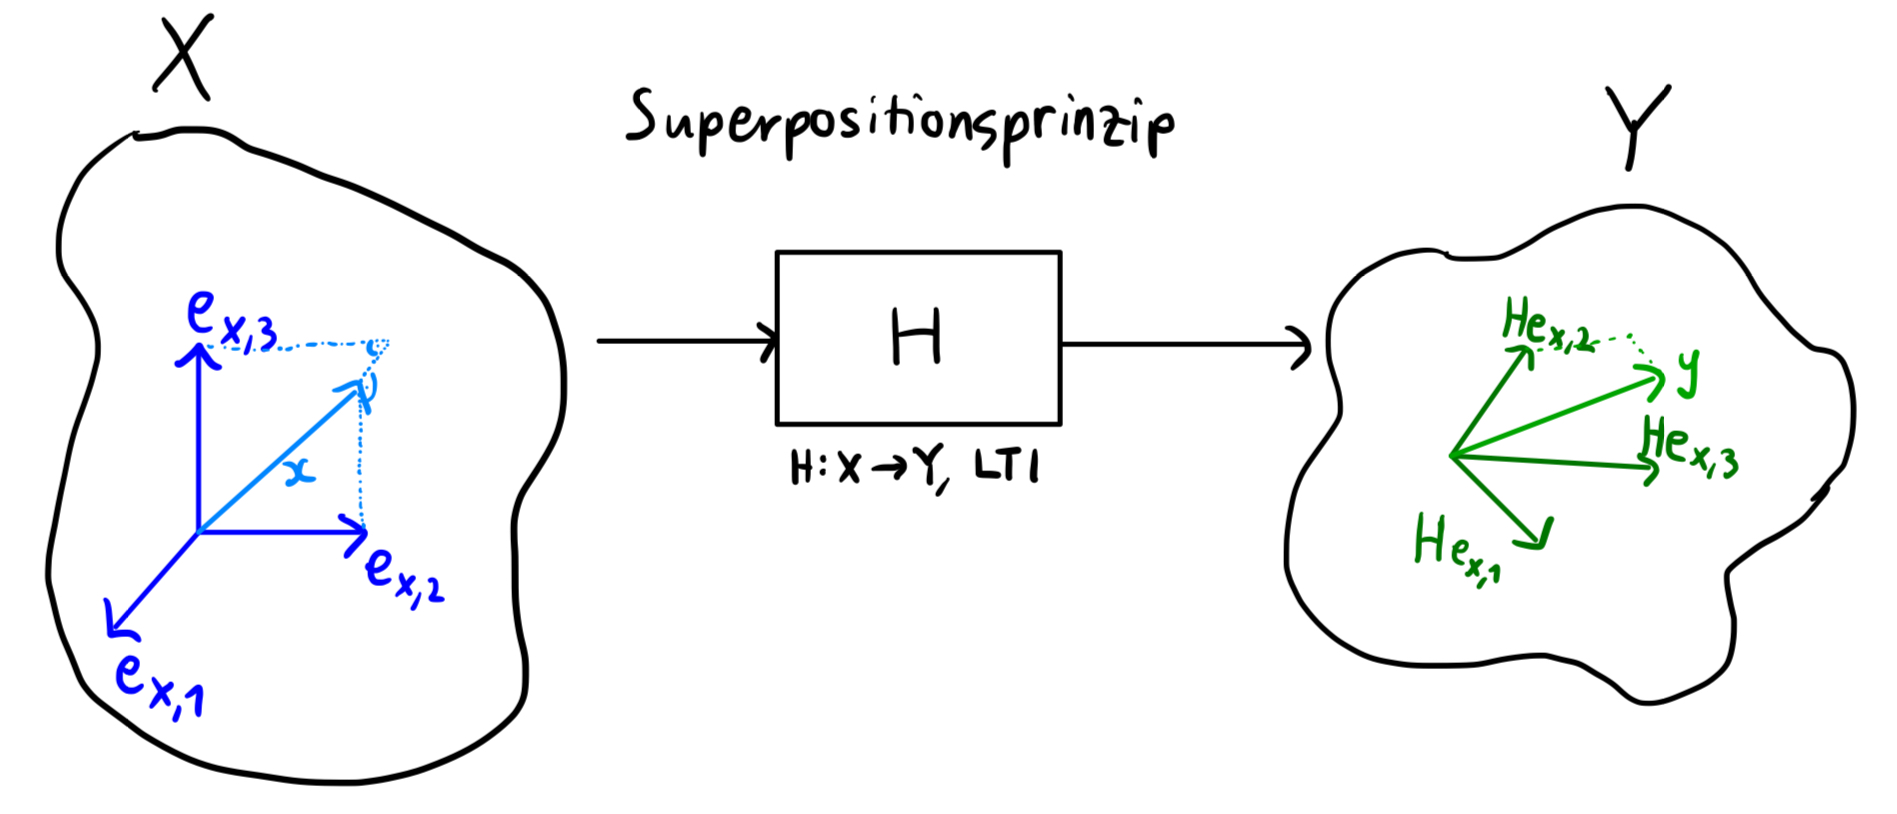
\includegraphics[width=0.8\linewidth]{docimgs/Superposition.jpeg}
    \end{center}
    \item[] Dies wird jedoch unmöglich, sobald die linearen Räume, auf denen $H$ definiert ist, unendlich dimensional sind.
    \item[] Es gilt aber folgende wichtige Eigenschaft, die uns ermöglicht, Systeme auf unendlichdimensionalen linearen Räumen zu charakterisieren.
\end{itemize}
\vspace*{-0.5cm}
\fcolorbox{darkblue}{lightblue}{\parbox{\dimexpr\linewidth-2\fboxsep-2\fboxrule\relax}{
\textbf{\begin{center}
    LTI-Systeme sind vollständig durch ihre Impulsantwort $h := (H \delta)(t)$ definiert.
\end{center}} 
}}%

Das heisst, wir können dem System einen $\delta-$Impuls als Input geben und den Output betrachten und dieser Output charakterisiert das LTI-System vollständig.


\vfill \null
\pagebreak

\vspace*{-0.5cm}
\subsection*{Herleitung}
\vspace*{-0.5cm}
\begin{itemize}[leftmargin=0pt]
    \item[] \textbf{Annahmen}: $x(t)$ sei absolut integrierbar, resp. $\displaystyle \int_{-\infty}^\infty |x(t)|\text{d}t < \infty$
\end{itemize}

\vspace*{-0.5cm}

\begin{tikzpicture}
    % Define the box size and grid spacing
    \draw[step=0.5cm,gray!50,very thin] (0,0) grid (16.5,17); % (0,0) is bottom-left corner, (10,10) is top-right corner
\end{tikzpicture}


\vfill \null
\pagebreak

\fcolorbox{darkblue}{lightblue}{\parbox{\dimexpr\linewidth-2\fboxsep-2\fboxrule\relax}{
\begin{center}
    Ein LTI-System antwortet auf ein Eingangssignal $x(t)$ mit dem Ausgangssignal
    $$y(t) = \int_{-\infty}^\infty x(\tau)h(t-\tau)\text{d}\tau := x \ast h$$
    wobei $h(t) = (H\delta)(t)$ die \textbf{Impulsantwort} des Systems ist.
\end{center}
}}%

$x \ast h$ nennt man die \textbf{Faltung} (englisch \textit{convolution}) von $x$ mit $h$. Es reicht also, eine einzige Messung $h(t) = (H \delta)(t)$ durchzuführen, um das System $H$ vollständig zu charakterisieren.

\vspace*{-0.5cm}
\subsubsection*{Bemerkung:}
\vspace*{-0.5cm}
System ist in der Form $y(t) = \displaystyle\int_{-\infty}^{\infty} x(\tau) h(t-\tau) \text{d}\tau$ darstellbar $\implies$ System ist ein LTI-System.
System ist ein LTI-System $\centernot{\implies}$ System ist in der Form $y(t) = \displaystyle\int_{-\infty}^{\infty} x(\tau) h(t-\tau) \text{d}\tau$ darstellbar.
\vspace*{-0.5cm}
\begin{itemize}[leftmargin=0pt]
    \item[] Das heisst es gibt auch LTI-Systeme, deren Ausgangssignal sich nicht als Faltung des Eingangssignals mit der Impulsantwort charakterisieren lässt, jedoch nicht umgekehrt.
    \item[] Wir werden aber in SST1 immer einfachheitshalber annehmen, dass wann immer wir ein LTI-System gegeben haben, dann handelt es sich um LTI-Systeme, die auch stetig sind und eine Darstellung der Form $y(t) = \displaystyle\int_{-\infty}^{\infty} x(\tau) h(t-\tau) \text{d}\tau$ haben.
\end{itemize}

\vspace*{-0.5cm}
\subsection*{Aufgabe 42.a)}
\vspace*{-0.5cm}
Ein LTI-System ist durch die folgende Eingangs-Ausgangsbeziehung beschrieben
$$y(t) = \int_{-\infty}^t \text{e}^{-(t-\tau)}x(\tau-2)\text{d}\tau$$
Bestimmen Sie die Impulsantwort des Systems.


\begin{tikzpicture}
    % Define the box size and grid spacing
    \draw[step=0.5cm,gray!50,very thin] (0,0) grid (16.5,5.5
    ); % (0,0) is bottom-left corner, (10,10) is top-right corner
\end{tikzpicture}

\pagebreak

\subsection*{Existenz des Faltungsintegrals und Eigenschaften der Faltung}
\vspace*{-0.5cm}
Es ist nicht immer garantiert, dass das Faltungsintegral zweier Signale $x_1(t)$ und $x_2(t)$, d.h. $$(x_1 \ast x_2)(t) = \int_{-\infty}^{\infty} x_1(\tau)x_2(t-\tau) \text{d}\tau$$ existiert. Die Young'sche Ungleichung stellt sicher, dass eine Faltung zweier Signale existiert. Zuerst jedoch ein bisschen Repetition:
\vspace*{-0.5cm}
\begin{itemize}[leftmargin = 0pt]
     \item[] $L^p$ ist der Raum aller Funktionen $x$, die $\displaystyle\int_{-\infty}^{\infty} |x(t)|^p \text{d}t < \infty$ erfüllen.
     \item[] Die $p-$Norm $||\cdot||_p$ ist gegeben durch $||x||_p := \left(\displaystyle\int_{-\infty}^{\infty} |x(t)|^p \text{d}t\right)^{1/p}$
     \item[] Spezialfall: $||x||_{\infty} := \inf\{C \geq 0: |x(t)| \leq C, \text{ für alle } t\in \mathbb{R}\}$.
     \item[] \textbf{Theorem:} \textit{(Young'sche Ungleichung)} 
     \item[] Seien $x$ und $h$ (messbare) Funktionen, sodass $||x||_p, \; ||h||_q < \infty$ für $p,q$ mit $1 \leq p,q \leq \infty$. Man setze:\\
     $$\frac{1}{p} + \frac{1}{q} = 1 + \frac{1}{r}$$
     Dann gilt: $||x \ast h||_r \leq ||x||_p||h||_q$.
     \item[] Zwei Spezialfälle, die aus der Young'schen Ungleichung folgen:
     \item[] $x_1 \in L^p, \; 1 \leq p \leq \infty, \; x_2 \in L^1 \implies ||x_1 \ast x_2 ||_p \leq ||x_1||_p ||x_2||_1$ und damit $x_1 \ast x_2 \in L^p$
     \item[] $x_1 \in L^2, \; x_2 \in L^2 \implies |(x_1 \ast x_2 )(t)| \leq ||x_1||_2 ||x_2||_2, \; t \in \mathbb{R}$ und damit $x_1 \ast x_2 \in L^\infty$
\end{itemize}

\subsubsection*{Eigenschaften der Faltung}
\begin{enumerate}
    \item kommutativ: $x_1 \ast x_2 = x_2 \ast x_1$
    \item assoziativ: $x_1 \ast (x_2 \ast x_3) = (x_1 \ast x_2) \ast x_3$
    \item distributiv: $x_1 \ast (x_2 + x_3) = x_1 \ast x_2 + x_1 \ast x_3$
    \item linear in beiden Argumenten: $x_1 \ast (\alpha x_2 + \beta x_3) = \alpha (x_1 \ast x_2) + \beta (x_1 \ast x_3)$
\end{enumerate}

\subsection*{Interpretation des Faltungsintegrals}
\vspace*{-0.5cm}
Man kann das Faltungsintegral als eine gewichtete Linearkombination zeitverschobener Versionen des Eingangssignals verstehen. Die Gewichtungskoeffizienten sind durch die Impulsantwort $h(t)$ gegeben.
Die Faltung kann man entweder analytisch oder graphisch berechnen.

\vfill \null
\pagebreak

%\vspace*{-0.5cm}
\subsubsection*{Analytisch: Aufgabe 41}
\vspace*{-0.5cm}
Für die Signale $x_1(t) = e^{-\alpha t}\sigma(t)$ und $x_2(t) = e^{-\beta t}\sigma(t)$ berechne man die Faltung $y(t) = (x_1 \ast x_2)(t)$ (auch für $\alpha = \beta$!).


\begin{tikzpicture}
    % Define the box size and grid spacing
    \draw[step=0.5cm,gray!50,very thin] (0,0) grid (16.5,5
    ); % (0,0) is bottom-left corner, (10,10) is top-right corner
\end{tikzpicture}

\fcolorbox{darkblue}{lightblue}{%
\parbox{\dimexpr\linewidth-2\fboxsep-2\fboxrule\relax}{\begin{itemize}
    \item[] \textbf{Graphische Faltung: Kochrezept}
    \item[] \textbf{Ziel}: Wir wollen $y(t) = \displaystyle\int_{-\infty}^{\infty} x(t-\tau)h(\tau) \text{d}\tau$ berechnen.
    \item[1)] $x(\tau)$ spiegeln um $\tau = 0$, um $x(-\tau)$ zu erhalten.
    \item[2)] Das gespiegelte $x(\tau)$ um $t$ verschieben.
    \item[] \begin{multicols}{2}
        \begin{itemize}
        \item nach rechts für $t>0$
        \item[] $\implies x(t -\tau) = x(-(\tau-t))$
        \item nach links für $t<0$
    \end{itemize}
    \end{multicols}
    \item[3)] Das gespiegelte \& verschobene $x(\tau)$ mit $h(\tau)$ multiplizieren. $\implies x(t-\tau)h(\tau)$
    \item[4)] Integrieren \& den Wert von $y(t)$ bei $t$ eintragen.
    \item[5)] Zurück zu 2) mit neuem $t$. Wir führen die Integration in 4) an jeder Stelle erneut durch, wo sich das Verhalten von $x(t-\tau)$ zu $h(\tau)$ sprungartig verändert.
\end{itemize}
\textbf{Hinweise}: Vergesst nicht, dass die Faltung kommutativ ist, d.h.
$$\int_{-\infty}^\infty x(t-\tau) h(\tau) \text{d}\tau = \int_{-\infty}^\infty x(\tau) h(t-\tau) \text{d}\tau$$
Manchmal ist es sinnvoller, $h(\tau)$ anstatt $x(\tau)$ zu spiegeln und zu verschieben. In der Regel verschiebt man das einfachere Signal und fixiert das kompliziertere Signal.
}}%
\vfill \null
\pagebreak

\subsection*{Aufgabe 39.a)}
\vspace*{-0.5cm}
Bestimmen Sie $x_1 \ast x_2$ für die angegebenen Signale $x_1$ und $x_2$.

\vspace*{-0.5cm}
\begin{center}
    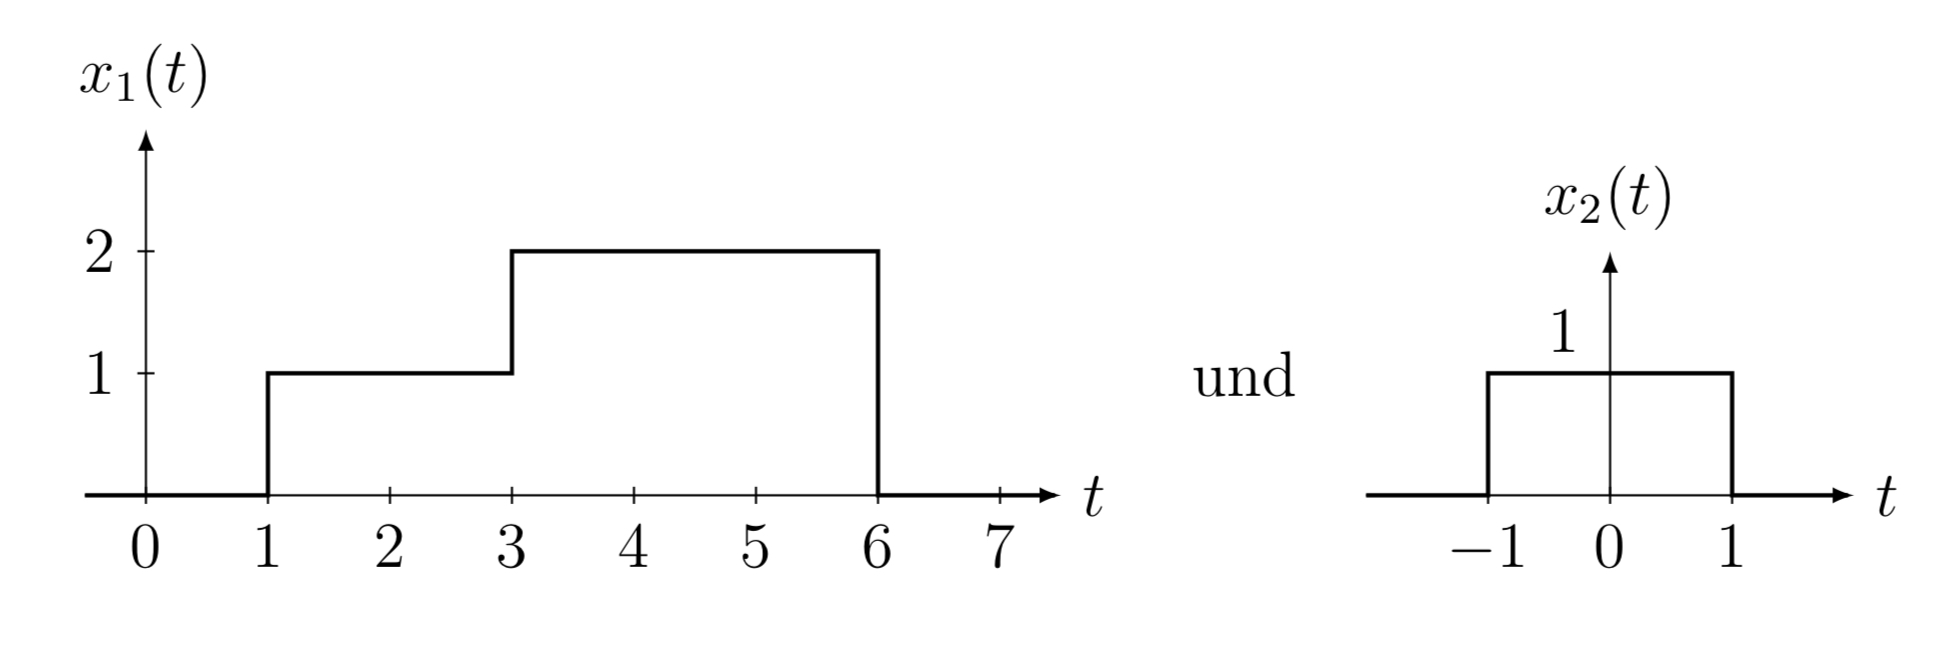
\includegraphics[width=0.7\linewidth]{docimgs/ex39a.jpg}
\end{center}
\vspace*{-0.5cm}


\begin{tikzpicture}
    % Define the box size and grid spacing
    \draw[step=0.5cm,gray!50,very thin] (0,0) grid (16.5,15
    ); % (0,0) is bottom-left corner, (10,10) is top-right corner
\end{tikzpicture}

\pagebreak

\subsection*{Eigenschaften der Impulsantwort}
\vspace*{-0.5cm}
Gegeben ist ein LTI-System mit der Eingangs-Ausgangsbeziehung $$y(t) = (Hx)(t) = \displaystyle\int_{-\infty}^{\infty} h(\tau)x(t-\tau)\text{d}\tau =  \displaystyle\int_{-\infty}^{\infty} x(\tau)h(t-\tau)\text{d}\tau$$

\fcolorbox{darkblue}{lightblue}{%
\parbox{\dimexpr\linewidth-2\fboxsep-2\fboxrule\relax}{
%\vspace*{-0.5cm}
\subsubsection*{Kausalität}
Ein LTI-System ist kausal dann und nur dann, wenn
$h(t) = 0 \text{ für } t < 0.$
\vspace*{1cm}
\subsubsection*{Gedächtnislosigkeit}
Ein LTI-System $H$ ist gedächtnislos, wenn für alle $x(t)$ und alle Zeitpunkte $t_0 \in \mathbb{R}$ das Ausgangssignal $(Hx)(t)$ zum Zeitpunkt $t_0$, d.h. $(Hx)(t_0)$, nur von $x(t_0)$ abhängt. Da das System linear sein muss (wir betrachten ja LTI-Systeme), muss die Eingangs-Ausgangsbeziehung notwendigerweise folgende Form haben:
$$y(t) = (Hx)(t) = \alpha x(t), \hspace{10pt} \alpha \in \mathbb{C}$$
Das ist gleichbedeutend wie wenn wir sagen, dass die Impulsantwort die Form $h(t) = \alpha \delta(t)$ hat.
\vspace*{1cm}
\subsubsection*{BIBO-Stabilität}
%\vspace*{-0.5cm}
Wenn $h \in L^1$, dann ist das LTI-System BIBO-stabil.
}}%

\vfill \null
\pagebreak

\subsection*{Aufgabe 45}
\vspace*{-0.5cm}
Ein LTI-System sei durch die Impulsantwort $$h(t) = \sigma\left(\frac{t}{2} + 1\right) - \sigma\left(\frac{t}{2}-1\right)$$ beschrieben, wobei $\sigma(t)$ die Sprungfunktion bezeichnet.
\vspace*{-0.5cm}
\begin{itemize}
    \item[a)] Skizzieren Sie den Zeiterlauf der Impulsantwort $h(t)$.
    \item[b)] Ist das System (begründen Sie ihre Antworten!)
    \begin{multicols}{3} \begin{itemize}
            \item[i)] kausal?
            \item[ii)] gedächtnisbehaftet?
            \item[iii)] BIBO-stabil?
        \end{itemize}
    \end{multicols}
    \item[c)] Bestimmen Sie die Antwort $y(t)$ des Systems auf das Eingangssignal $x(t)= e^{-t}\sigma(t)$
\end{itemize}


\begin{tikzpicture}
    % Define the box size and grid spacing
    \draw[step=0.5cm,gray!50,very thin] (0,0) grid (16.5,14
    ); % (0,0) is bottom-left corner, (10,10) is top-right corner
\end{tikzpicture}

\pagebreak


\begin{tikzpicture}
    % Define the box size and grid spacing
    \draw[step=0.5cm,gray!50,very thin] (0,0) grid (16.5,20
    ); % (0,0) is bottom-left corner, (10,10) is top-right corner
\end{tikzpicture}

\pagebreak

\subsection*{Prüfungsaufgabe: Frühjahr 2024, Aufgabe 1}
\vspace*{-0.5cm}
Ein analoges LTI-System sei durch folgende Eingangs-Ausgangsbeziehung beschrieben:
$$y(t) = \int_{-\infty}^t e^{-4(t-\tau)}x(\tau)\text{d}\tau.$$
\begin{itemize}
    \item[$\star$ (a)] (3 Punkte) Bestimmen Sie die Impulsantwort des Systems.
    \item[$\star$ (b)] (2 Punkte) Ist das System kausal? Begründen Sie Ihre Antwort.
    \item[$\star$ (c)] (2 Punkte) Ist das System BIBO-stabil? Begründen Sie Ihre Antwort.
    \item[$\star$ (d)] (4 Punkte) Bestimmen Sie die Antwort des Systems auf das Eingangssignal \\$x_1(t) = \sigma(t) - \sigma(t-2).$
    \item[$\star$ (e)] (4 Punkte) Bestimmen Sie die Antwort des Systems auf das abgebildete Signal $x_2(t).$
\end{itemize}
\vspace*{-1cm}
\begin{center}
    \includegraphics[width=0.7\linewidth]{docimgs/ex_exam21_frühjahr_1.jpeg}
\end{center}
\vspace*{-0.5cm}
\textit{Hinweis: Diese Teilaufgabe kann effizient unter Verwendung des Ergebnisses aus Teilaufgabe d) gelöst werden.}


\begin{tikzpicture}
    % Define the box size and grid spacing
    \draw[step=0.5cm,gray!50,very thin] (0,0) grid (16.5,6
    ); % (0,0) is bottom-left corner, (10,10) is top-right corner
\end{tikzpicture}

\pagebreak


\begin{tikzpicture}
    % Define the box size and grid spacing
    \draw[step=0.5cm,gray!50,very thin] (0,0) grid (16.5,20
    ); % (0,0) is bottom-left corner, (10,10) is top-right corner
\end{tikzpicture}

\end{document}